\documentclass[11pt]{tg_usta}
\labelpaper[year =2026 , month =6]
\usepackage{anysize}
\marginsize{1in}{1in}{1in}{1in}
\usepackage{amsmath,amsthm,amssymb}
\usepackage{graphicx}
\usepackage{booktabs}
\usepackage{url}
\usepackage{array}
\decimalpoint

\begin{document}
\title[maintitle = Proyecto Centinela --- Fase 1: línea base con un MLP,
       secondtitle = Sistema de alerta temprana del poder adquisitivo del salario mínimo (Bogotá),
       shorttitle = Centinela Fase 1 --- MLP]

\begin{authors}
\author[firstname = Estefanny,
        surname = Ruíz González,
        affiliation = {Estudiante},
        email = estefannyruiz@usantotomas.edu.co]
\author[firstname = Miguel,
        surname = Alarcón Ojeda,
        affiliation = {Estudiante},
        email = miguel.alarcon@usantotomas.edu.co]
\end{authors}

\section{Problema, contexto y cliente}

El poder adquisitivo real del salario mínimo legal vigente (SMLV) se erosiona cuando la inflación crece más rápido que el ajuste nominal del salario. Esta pérdida no siempre es perceptible de inmediato y suele reconocerse cuando ya ha afectado el consumo de los hogares. Este trabajo construye la línea base de un sistema de alerta temprana (``Centinela'') que predice si el poder adquisitivo del SMLV \textbf{está cayendo} en un mes dado, definido como una variación anual negativa del salario real. El \textbf{cliente} es un analista de política pública o de un gremio laboral que requiere una señal objetiva de erosión del salario para sustentar decisiones de ajuste con anticipación. El proyecto se enmarca en la investigación de grado de los autores (poder adquisitivo del SMLV), con Bogotá como ciudad piloto antes de generalizar a las áreas metropolitanas del DANE.

La tarea conecta con el Módulo I del curso: un perceptrón multicapa (MLP) supervisado sobre datos tabulares, entrenado desde cero, con clasificación binaria mediante una salida sigmoide. La serie económica mensual, aplanada a tabla, constituye la modalidad de esta fase; la modalidad secuencial (procesamiento con redes recurrentes) se reserva para la Fase 2.

\section{Datos y metodología}

La base fue consolidada manualmente por los autores a partir de fuentes oficiales (DANE para el IPC de Bogotá; Banco de la República para la TRM; Ministerio de Trabajo/DANE para el SMLV), sin recurrir a Kaggle ni a sus réplicas \cite{dane2025,banrep2025}. Comprende 324 registros mensuales (enero 2000 -- diciembre 2026); los meses finales de 2026 son proyectados, lo que se declara como limitación.

\textbf{Variable objetivo.} \texttt{riesgo} $= 1$ si la variación anual del salario real es negativa; $0$ en caso contrario. El análisis exploratorio reveló un fuerte \textbf{desbalance de clases}: solo 30 de 324 meses (9.3\,\%, equivalente al 9.6\,\% sobre los datos utilizables) corresponden a la clase de riesgo. Este hallazgo es la decisión metodológica central: la exactitud global resulta engañosa --un clasificador trivial que prediga siempre ``sin riesgo'' acertaría $\sim$90\,\%--, por lo que la evaluación se basa en \emph{recall} y F1 de la clase de riesgo.

\textbf{Ingeniería de variables y fuga de datos.} Las variables en su nivel crudo (IPC, TRM, salario nominal) mostraron correlación casi nula con la etiqueta ($\pm0.06$). En cambio, las variables de \textbf{dinámica} sí aportan señal: variación mensual y trimestral del IPC (\texttt{ipc\_mom}, \texttt{ipc\_mom3}) y la brecha entre el crecimiento anual del salario nominal y la inflación (\texttt{brecha\_yoy}), con correlaciones de 0.33 a 0.37. La selección tiene fundamento económico directo: el salario real cae cuando el nominal crece menos que los precios. Se excluyeron explícitamente \texttt{smlv\_real}, \texttt{smlv\_real\_var\_anual} y \texttt{poder\_adq\_index} como variables de entrada, por ser la base de la etiqueta (la tercera es \texttt{smlv\_real} reescalado a base 100); su inclusión habría constituido fuga de datos.

\textbf{Partición.} Por tratarse de una serie temporal, la partición train/val/test es \textbf{cronológica 70/15/15} (no aleatoria), evitando que el modelo acceda a información futura. El EDA mostró que los casos de riesgo se concentran en periodos históricos, dejando el conjunto de prueba más reciente (2023--2026) \textbf{sin casos positivos}. Conservando el orden cronológico, las métricas de detección se reportan sobre el conjunto de \textbf{validación} (2019--2023), que contiene 13 casos de riesgo. El escalado (estandarización) se ajustó únicamente con el conjunto de entrenamiento.

\section{Modelo y entrenamiento}

El modelo es un MLP con dos capas ocultas (16 y 8 neuronas) y activación ReLU. La salida es una única neurona sin activación (logit); la sigmoide se integra en la función de pérdida \texttt{BCEWithLogitsLoss} por estabilidad numérica, evitando el antipatrón de doble sigmoide. Para contrarrestar el desbalance se aplicó \texttt{pos\_weight}, que pondera el error sobre la clase minoritaria ($\sim$12$\times$). El entrenamiento usa un bucle explícito de 50 épocas (\texttt{zero\_grad} $\rightarrow$ \texttt{forward} $\rightarrow$ pérdida $\rightarrow$ \texttt{backward} $\rightarrow$ \texttt{step}) con optimizador Adam ($lr = 0.01$) y semilla fija para reproducibilidad.

\begin{figure}[!ht]
\centering
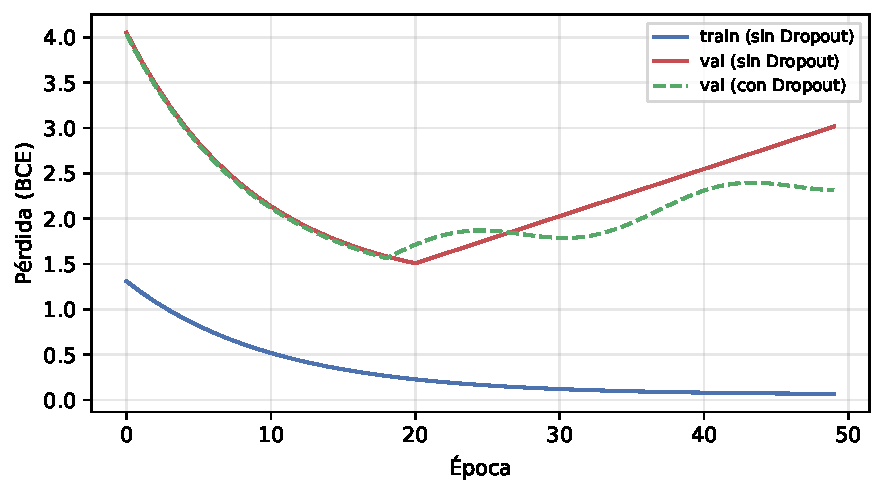
\includegraphics[width=0.72\textwidth]{curvas_perdida.pdf}
\caption{Curvas de pérdida. La pérdida de entrenamiento desciende de forma sostenida mientras la de validación (sin Dropout) repunta a partir de la época $\sim$20: sobreajuste. La variante con Dropout mantiene la validación más estable.}
\label{fig:curvas}
\end{figure}

\textbf{Regularización.} Se entrenó un segundo modelo idéntico con Dropout ($p = 0.30$). La comparación (Figura~\ref{fig:curvas}) evidencia que el modelo base memoriza el entrenamiento y generaliza peor tras la época $\sim$20, mientras que el Dropout retrasa y atenúa ese deterioro. El punto de menor pérdida de validación define el criterio de selección de época.

\section{Resultados}

Sobre el conjunto de validación ($n=47$), el modelo con Dropout obtuvo los resultados de la Tabla~\ref{tab:metricas} y la matriz de confusión de la Figura~\ref{fig:matriz}.

\begin{table}[h]
\centering
\begin{tabular}{lc}
\toprule
\textbf{Métrica (clase riesgo)} & \textbf{Valor} \\
\midrule
Precisión & 0.917 \\
Recall    & 0.846 \\
F1        & 0.880 \\
\bottomrule
\end{tabular}
\caption{Métricas sobre el conjunto de validación.}
\label{tab:metricas}
\end{table}

\begin{figure}[!ht]
\centering
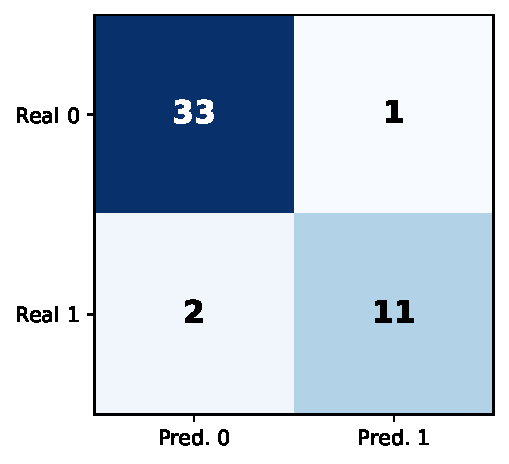
\includegraphics[width=0.42\textwidth]{matriz_confusion.pdf}
\caption{Matriz de confusión (validación, $n=47$). Filas: clase real; columnas: clase predicha.}
\label{fig:matriz}
\end{figure}

De 13 casos de riesgo reales, el modelo detectó 11 (recall 0.85), con un solo falso positivo y dos falsos negativos. Para una línea base sobre datos fuertemente desbalanceados, el resultado es prometedor: el uso de \texttt{pos\_weight} evitó que el modelo ignorara la clase minoritaria. Estos valores deben leerse con cautela dada la escala reducida del conjunto de validación (47 meses); constituyen evidencia de viabilidad, no una garantía de desempeño en producción.

\section{Análisis ético}

En un sistema de alerta temprana, los dos errores tienen costos asimétricos. Un \textbf{falso negativo} (no avisar de una caída real del poder adquisitivo) priva al tomador de decisiones de margen de reacción y perpetúa la pérdida de bienestar de los hogares dependientes del SMLV; es el error más costoso. Un \textbf{falso positivo} (alertar sin causa) genera un costo menor --decisiones o alarma sin fundamento y desgaste de credibilidad--. Coherente con esta valoración, el diseño priorizó minimizar falsos negativos (maximizar recall) mediante \texttt{pos\_weight}; el resultado (solo 2 falsos negativos) refleja esa intención. Esta priorización se alinea con el Marco Ético para la Inteligencia Artificial en Colombia \cite{minciencias2021}, que antepone el impacto real sobre las personas a la exactitud agregada. Como salvaguarda, el sistema se concibe como apoyo a la decisión experta, no como su sustituto.

\section{Limitaciones y trabajo futuro}

\begin{itemize}
\item \textbf{Muestra y alcance.} $\sim$312 meses utilizables y una sola ciudad (Bogotá); los resultados no son directamente generalizables a otras regiones, donde la dinámica de precios difiere. Parte de 2026 es proyectada.
\item \textbf{Índice de asequibilidad (Brecha).} Siguiendo la recomendación de la asesora del proyecto de grado, una extensión valiosa es incorporar la relación entre el costo de la canasta básica y el SMLV como variable adicional de bienestar, contrastando IPC y canastas regionales de forma independiente.
\item \textbf{Agrupamiento por dinámica temporal.} También por sugerencia de la asesora, para la fase multi-ciudad se propone un agrupamiento jerárquico basado en \emph{Dynamic Time Warping} (DTW), que alinea series con choques inflacionarios desfasados en el tiempo y permitiría construir modelos por clúster de ciudades funcionalmente similares en lugar de un modelo aislado por ciudad.
\item \textbf{Modalidad secuencial.} La Fase 2 procesará la serie con redes recurrentes (RNN/LSTM/GRU) que exploten la dependencia temporal que el aplanamiento tabular descarta.
\end{itemize}

\renewcommand{\refname}{Referencias}
\begin{thebibliography}{9}
\harvarditem{Banco de la República}{2025}{banrep2025} Banco de la República (2025). \emph{Tasa de cambio representativa del mercado (TRM)}. Bogotá. \url{https://www.banrep.gov.co}
\harvarditem{DANE}{2025}{dane2025} Departamento Administrativo Nacional de Estadística (DANE) (2025). \emph{Índice de Precios al Consumidor (IPC)}. Bogotá. \url{https://www.dane.gov.co/index.php/estadisticas-por-tema/precios-y-costos/indice-de-precios-al-consumidor-ipc}
\harvarditem{Minciencias}{2021}{minciencias2021} Ministerio de Ciencia, Tecnología e Innovación (Minciencias) (2021). \emph{Marco Ético para la Inteligencia Artificial en Colombia}. Gobierno de Colombia.
\end{thebibliography}

\end{document}
